% Options for packages loaded elsewhere
\PassOptionsToPackage{unicode}{hyperref}
\PassOptionsToPackage{hyphens}{url}
%
\documentclass[
  11pt,
  ignorenonframetext,
]{beamer}
\usepackage{pgfpages}
\setbeamertemplate{caption}[numbered]
\setbeamertemplate{caption label separator}{: }
\setbeamercolor{caption name}{fg=normal text.fg}
\beamertemplatenavigationsymbolsempty
% Prevent slide breaks in the middle of a paragraph
\widowpenalties 1 10000
\raggedbottom
\setbeamertemplate{part page}{
  \centering
  \begin{beamercolorbox}[sep=16pt,center]{part title}
    \usebeamerfont{part title}\insertpart\par
  \end{beamercolorbox}
}
\setbeamertemplate{section page}{
  \centering
  \begin{beamercolorbox}[sep=12pt,center]{part title}
    \usebeamerfont{section title}\insertsection\par
  \end{beamercolorbox}
}
\setbeamertemplate{subsection page}{
  \centering
  \begin{beamercolorbox}[sep=8pt,center]{part title}
    \usebeamerfont{subsection title}\insertsubsection\par
  \end{beamercolorbox}
}
\AtBeginPart{
  \frame{\partpage}
}
\AtBeginSection{
  \ifbibliography
  \else
    \frame{\sectionpage}
  \fi
}
\AtBeginSubsection{
  \frame{\subsectionpage}
}
\usepackage{amsmath,amssymb}
\usepackage{lmodern}
\usepackage{iftex}
\ifPDFTeX
  \usepackage[T1]{fontenc}
  \usepackage[utf8]{inputenc}
  \usepackage{textcomp} % provide euro and other symbols
\else % if luatex or xetex
  \usepackage{unicode-math}
  \defaultfontfeatures{Scale=MatchLowercase}
  \defaultfontfeatures[\rmfamily]{Ligatures=TeX,Scale=1}
\fi
\usetheme[]{metropolis}
% Use upquote if available, for straight quotes in verbatim environments
\IfFileExists{upquote.sty}{\usepackage{upquote}}{}
\IfFileExists{microtype.sty}{% use microtype if available
  \usepackage[]{microtype}
  \UseMicrotypeSet[protrusion]{basicmath} % disable protrusion for tt fonts
}{}
\makeatletter
\@ifundefined{KOMAClassName}{% if non-KOMA class
  \IfFileExists{parskip.sty}{%
    \usepackage{parskip}
  }{% else
    \setlength{\parindent}{0pt}
    \setlength{\parskip}{6pt plus 2pt minus 1pt}}
}{% if KOMA class
  \KOMAoptions{parskip=half}}
\makeatother
\usepackage{xcolor}
\newif\ifbibliography
\usepackage{graphicx}
\makeatletter
\def\maxwidth{\ifdim\Gin@nat@width>\linewidth\linewidth\else\Gin@nat@width\fi}
\def\maxheight{\ifdim\Gin@nat@height>\textheight\textheight\else\Gin@nat@height\fi}
\makeatother
% Scale images if necessary, so that they will not overflow the page
% margins by default, and it is still possible to overwrite the defaults
% using explicit options in \includegraphics[width, height, ...]{}
\setkeys{Gin}{width=\maxwidth,height=\maxheight,keepaspectratio}
% Set default figure placement to htbp
\makeatletter
\def\fps@figure{htbp}
\makeatother
\setlength{\emergencystretch}{3em} % prevent overfull lines
\providecommand{\tightlist}{%
  \setlength{\itemsep}{0pt}\setlength{\parskip}{0pt}}
\setcounter{secnumdepth}{-\maxdimen} % remove section numbering
\ifLuaTeX
  \usepackage{selnolig}  % disable illegal ligatures
\fi
\IfFileExists{bookmark.sty}{\usepackage{bookmark}}{\usepackage{hyperref}}
\IfFileExists{xurl.sty}{\usepackage{xurl}}{} % add URL line breaks if available
\urlstyle{same} % disable monospaced font for URLs
\hypersetup{
  pdftitle={Intervalos de confianza Poisson y Binomial},
  pdfauthor={Gerardo Martín},
  hidelinks,
  pdfcreator={LaTeX via pandoc}}

\title{Intervalos de confianza Poisson y Binomial}
\author{Gerardo Martín}
\date{2022-06-29}

\begin{document}
\frame{\titlepage}

\hypertarget{diferencias-con-distribuciuxf3n-normal}{%
\section{Diferencias con distribución
normal}\label{diferencias-con-distribuciuxf3n-normal}}

\begin{frame}{Normal}
\protect\hypertarget{normal}{}
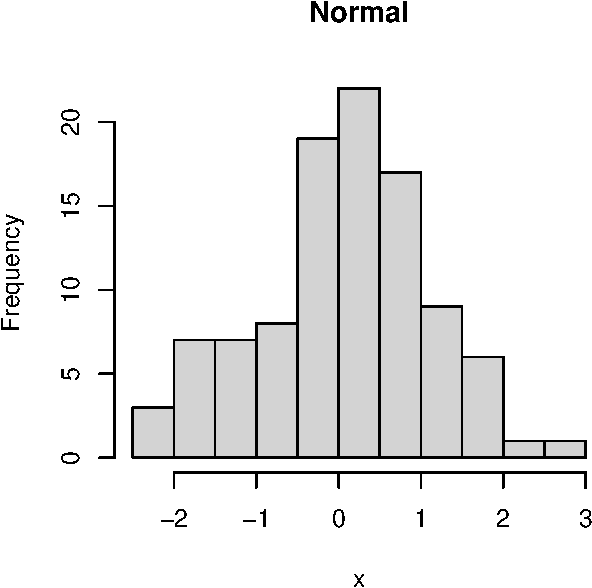
\includegraphics{Intervalos-poisson_files/figure-beamer/unnamed-chunk-1-1.pdf}
\end{frame}

\begin{frame}{Poisson}
\protect\hypertarget{poisson}{}
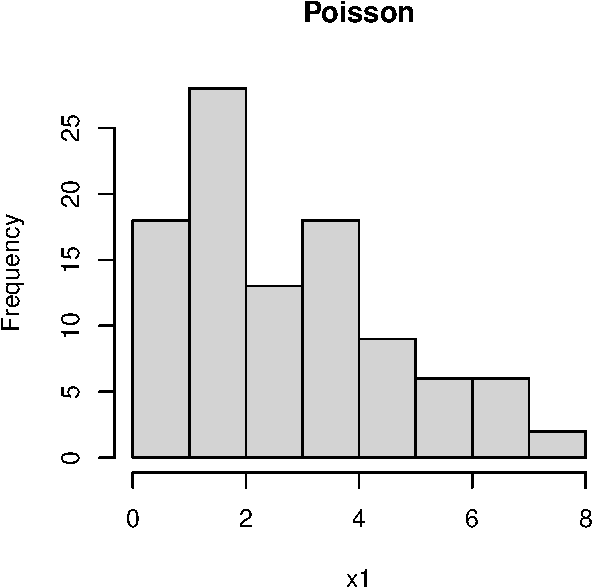
\includegraphics{Intervalos-poisson_files/figure-beamer/unnamed-chunk-2-1.pdf}
\end{frame}

\begin{frame}{Binomial}
\protect\hypertarget{binomial}{}
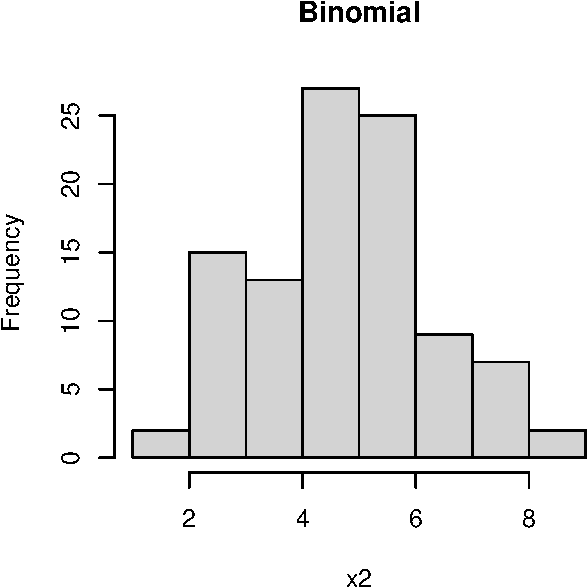
\includegraphics{Intervalos-poisson_files/figure-beamer/unnamed-chunk-3-1.pdf}
\end{frame}

\begin{frame}{Normal}
\protect\hypertarget{normal-1}{}
La fórmula es:

\[IC_{95} = \bar{x} \pm 1.96 \times \sigma/\sqrt{n}\]

Como sabemos, la distribución Poisson no es simétrica, por lo que este
método no funciona, y 1.96 no representa el número de desviaciones
estándar que acotan el 95\% de los datos.
\end{frame}

\begin{frame}{Poisson}
\protect\hypertarget{poisson-1}{}
\begin{itemize}
\item
  Inferior: \(0.5 \chi^2_{2 \times n, \alpha/2}\)
\item
  Superior: \(0.5 \chi^2_{2 \times (n+1), 1-\alpha/2}\)
\end{itemize}

Donde:

\begin{enumerate}
\tightlist
\item
  \(\chi^2\) es el estadístico chi cuadrada (más tarde para el cálculo)
\item
  \(n\) es el número de eventos observados
\item
  \(\alpha\) es el nivel de significancia. Si el nivel es al 95\%,
  \(\alpha = 1-0.95 = 0.05\), si el nivel es al 99\%,
  \(\alpha = 1-0.99 = 0.01\)
\end{enumerate}
\end{frame}

\begin{frame}{Binomial}
\protect\hypertarget{binomial-1}{}
\begin{itemize}
\item
  Inferior:
\item
  Superior:
\end{itemize}
\end{frame}

\end{document}
